\documentclass[12pt]{article}
\renewcommand{\baselinestretch}{1.3} 
\usepackage[a4paper, total={6in, 8in}]{geometry}
\usepackage{amsmath}
\usepackage{amssymb}
\usepackage{witharrows}
\usepackage{lipsum}
\usepackage{indentfirst}
\usepackage{mathtools}
\usepackage{layout}
\usepackage{xcolor}
\usepackage{blindtext}
\usepackage{sidenotes}
\usepackage{multicol}
\usepackage{fancyhdr}
\usepackage{indentfirst}
\usepackage{hyperref}
\usepackage{natbib}
\usepackage{indentfirst}
\usepackage{mwe}
\usepackage{epigraph}
\usepackage[skip=10pt plus1pt]{parskip}
\WithArrowsOptions{displaystyle,tikz=blue}

\begin{document}
\pagenumbering{gobble}
\begin{titlepage}
	\centering
	\vspace{1cm}
	{\Large \textsc{``Mathematics: Analysis And Approaches" Extended Essay}\par}
	\vspace{1.5cm}
	{\huge\bfseries EE Title (still haven't figured a good one out)\par}
	\vspace{2cm}
	\vfill
	\vfill
	{\large \today, a word count\par}
\end{titlepage}

\clearpage
\pagenumbering{arabic}
\tableofcontents
\newpage

%%% NOTES TO SELF:
%%% maybe explain what opposite means on a circle
%%% assume the Cat doesn't move if the Swan is directly in the centre

\section{Introduction}
\subsection{Abstract}
The research question of this Mathematics Extended Essay is the following problem:

\emph{Imagine a Swan in a middle of a perfectly circular unit lake. Standing on the edge is a hungry Cat. The Cat is after the Swan and the Swan's goal is to escape. The best route is flight, and yet it can only take off from land. The Cat on land is 4 times faster than the Swan on water. Can the Swan escape the Cat and if yes, what trajectory does it need to follow?}

In investigating this question I first ensured that it has a solution, followed by formulating a 2-part trajectory and finally using differential equations and techonology to approximate the curve.

\section{Solution}
There are several versions of the problem with different species chasing eachother around, but alas I could not trace down the source. Versions of this problem can be found under the names of "A Lady And A Monster"\cite{ladyandmonster}, "Game Of Cat And Mouse"\cite{Catandmouse} and others. The general premise and numerical values stay the same across interpretations. 

My primary reason for choosing to focus on this specific problem came from my strong desire to find an analytical solution to a problem I saw in a YouTube video\cite{Catandmouse}, it has been on my radar for a while and I see the window of opportunity. I also enjoy spending my free time pondering problems, although they are usually of computer science ilk.  

The described problem can be described using the following variables, all of which will be introduced later.

\begin{tabular}{|l|l|}
\hline
\textbf{Variable} & \textbf{Purpose}\\
\hline
$r = 1$ & The radius of the lake\\
$d$ & Distance of the Swan from the edge\\
$D = r - d$ & Distance of the Swan from the center, magnitude of position\\
$V$ & Magnitude of the Swan's velocity\\
$V' = 4V$ & Magnitude of the Cat's velocity\\
$\omega$ & The angular velocity of the Swan\\
$\omega'$ & The angular velocity of the Cat\\
$V_\omega'$ & Swan's linear compensation for Cat's angular velocity\\
$V_\alpha$ & Swan's velocity component directed away from the cat\\
$_\theta$ & The apparent distance between the Cat and the Swan\\
\hline
\end{tabular}
\vspace{12pt}

Both animals are acting \textit{optimally}, so are choosing whichever option gives them the best result in the moment. In Cat's case it is trying to be closer to the Swan, so it will always choose to move towards a point on the shore, that has the least distance to the Swan. That entails that the Cat has to try and reduce the apparent distance of it and its prey. Swan, however, has a chance to strategise, I will explain his movement in more detail further.

\begin{center}
	\begin{tikzpicture}[scale=2]
		\draw (0,0) circle [radius=1];
	\end{tikzpicture}
\end{center}

\subsection{The Dash Distance}

The simplest strategy for the Swan is to swim towards the shore opposite the Cat in a straight line without ever changing direction direction. The time it takes the Swan will be $\frac{r}{V}$ and the time it takes the Cat to get to that point is $\frac{\pi r}{V'} = \frac{\pi r}{4V}$. Based on that it is not difficult to see that the Cat will outrun the Swan.

\begin{center}
$\begin{WithArrows}[jot=2ex]
\frac{\pi r}{V'} &< \frac{r}{V} \Arrow{$V' = 4V$}\\
\frac{\pi r}{4V} &< \frac{r}{V} \Arrow{$\square \times \frac{V}{r}$}\\
\frac{\pi}{4} &< 1
\end{WithArrows}$
\end{center}

We see that the just dashing to the edge won't work for the Swan if it's in the middle, but we can image alternatives conditions. Assume the Swan is such distance $d$ away from edge and directly opposite the Cat, so that it can safely reach the edge, what are the possible values of $d$? It can be expressed as $\frac{d}{V} < \frac{\pi r}{4V} \Leftrightarrow  d < \frac{\pi}{4}r$.

\subsection{The Freedom Circle}

Now the question is whether it is even possible to get to that point. We can turn our attention to the angular velocities of the animals, since both of them are moving around the circle. If the distance of the Swan from the center is $D = r - d$, the Swan has the angular velocity of $\omega = \frac{V}{D}$ and the Cat has angular velocity $\omega' = \frac{4V}{r}$. Notice how the velocity of the Cat is essentially constant, but the velocity of the Swan is controlled by it's distance from the edge $d$. Based on this we can solve for the distance from the edge, at which the Swan will be faster (in terms of it's angular velocity) than the Cat.

\begin{center}
$\begin{WithArrows}[jot=2ex]
\frac{V}{D} &> \frac{4V}{r} \Arrow{$\square^{-1}$}\\
\frac{D}{V} &< \frac{r}{4V} \Arrow{$\square \times {-V}$}\\
-D &> -\frac{r}{4} \Arrow{$D = r - d$}\\
d - r &> -\frac{r}{4} \Arrow{$\square + r$}\\
d &> r - \frac{r}{4}
\end{WithArrows}$
\end{center}

Based on that we conclude that there exists an inner circle with radius $r - \frac{r}{4}$ in which the Swan can occupy \textit{any} position with any corresponding Cats position. %I am technically conjecturing this, do I need a more formal proof?}
That inner circle will be called the "freedom" circle.

Notice that there can exist such $d$ that $r - \frac{r}{4} < d < \frac{\pi}{4}r$. Given that $r = 1$ we get to know that the distance of the Swan from the edge has to be $\frac{3}{4} < d < \frac{3.14\dots}{4}$. The set of all positions for the Swan to be in forms an "safety" annulus inside the circle. When the Swan is inside this annulus and the Cat is opposite the Swan, it may dash to the edge of the lake and flee, so the trajectory must exist.

There exists an infinite amount of viable trajectories, since for every possible trajectory, the Swan can make a lap inside the "freedom" circle one more time, giving us a new trajectory. 

\subsection{Describing Velocity}

Next we may look at getting to the edge of the "safety" annulus. For a successful escape the Swan has to exit it at such point, that it's directly opposite the Cat. Over an infinitesimal amount of time $\Delta t$ the Swan can travel a total distance of $s = V \Delta t$. Assume the Swan is somewhere inside the "freedom" circle, then the Cat moves at $\omega' = \pm \frac{4V}{r}$. The Cat can move either clockwise or counterclockwise, since at all times there are two paths to its desired point and the Cat is always going to choose the shortest (except for the case when cat is directly opposite, since then two paths have equal lengths, when that happens we will assume the cat to move counterclockwise $\omega' > 0$).

In this case in order to compensate for the Cat's movement (remain opposite to it) the Swan has to move the same angle in the opposite direction. Since the magnitude of the velocity vector should remain $V$, we can express it as two vectors: moving away from the center to exit the "freedom" circle ($V_\alpha$) and compensation for Cat's movement ($V_{\omega'}$). If compensation is $V_{\omega'} = \omega' \times D$, we can solve for the away velocity ($V_\alpha$) as follows:

\begin{center}
$\begin{WithArrows}[jot=2ex]
V &= \sqrt{(\omega'D)^2  + V_\alpha^2} \Arrow{$\square^2$}\\
V^2 &= (\omega'D)^2  + V_\alpha^2 \Arrow{$\square - (\omega'D)^2$}\\
V_\alpha^2 &= V^2 - (\omega'D)^2 \Arrow{$\sqrt{\square}$}\\
V_\alpha &= \sqrt{V^2 - (\omega'D)^ 2}
\end{WithArrows}$
\end{center}

\begin{center}
	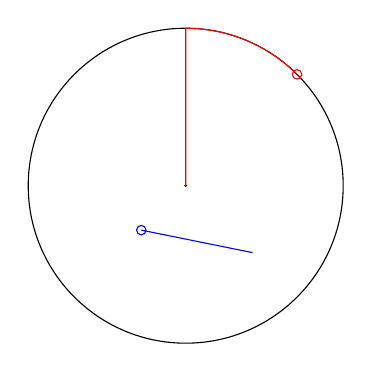
\begin{tikzpicture}[scale=2]
		\draw (0,0) circle [radius=1];
		\fill[color=black] (0,0) circle [radius=0.01];
		\draw[color=red] (0.707,0.707) circle [radius=0.03];
		\draw[color=blue] (-0.282,-0.282) circle [radius=0.03];
		\draw[color=red] (0.707,0.707) 
		arc[start angle = 45, end angle = 90, radius=1]
		(0, 0) -- (0, 1);
		\draw[color=blue] (-0.282, -0.282) -- (0.425, -0.425);
		
	\end{tikzpicture}
\end{center}

\subsection{Lake Shapes \& Polar Curves}

Since the case of a circular lake is solved we may generalize the problem to a broader case, specifically the case of any lake shape.

\subsection{Describing Position}

We can introduce a polar coordinate system to get the velocities for the Swan or the Cat as vectors ($V_\imath$ and $V'_\imath$ respectively) in the complex plane. Since the Cat always moves tangentially, it's velocity will always be directed at $\theta + \pi$. 

\begin{equation*}
\begin{WithArrows}[jot=2ex]
V'_{\imath} &= 4 \times \left\{ \begin{aligned} 
e^{i \times \frac{4V}{r}} \text{ when } \theta \geq 0 \\
e^{-i \times \frac{4V}{r}} \text{ when } \theta < 0\\
\end{aligned} \right.  %\Arrow{Trigonometric identities}\\
%V'_{\imath} &= \left\{ \begin{aligned} 
%-\cos(\theta) - \imath \sin(\theta)\\
%-\cos(\theta) - \imath \sin(\theta)\\
\end{WithArrows}
\end{equation*}

\section{Conclusion}
Glad I did it with \LaTeXe\cite{latex2e}, will continue using it.

\bibliographystyle{plain}
\bibliography{sources}
\end{document}
